\chapter{SOFTWARE USER GUIDE}

This appendix provides a practical guide for using the Inventory Management web application. It is written for daily users such as administrators, product controllers, purchasing staff, sales staff, and finance staff. The guide follows the same business workflow used by the system: prepare master data, create quotations, buy from suppliers, sell to customers, follow up billing and payments, and review the business situation.

\section{Starting the Software}

The software can be started in two main ways. The recommended approach for demonstration is Docker Compose because it starts the MySQL database, Django backend API, and React/Vite frontend together. Manual startup can also be used when the developer wants to run each service directly on the local machine.

\subsection{Starting with Docker Compose}

Before starting, Docker Desktop should be installed and running. From the project root directory, run the following command:

\begin{verbatim}
docker compose up --build
\end{verbatim}

The first startup may take a few minutes because Docker needs to download images and build the application containers. When startup is complete, open the frontend application in a browser:

\begin{verbatim}
http://127.0.0.1:5173/
\end{verbatim}

The backend API and Django admin are available at:

\begin{verbatim}
http://127.0.0.1:8000/api/
http://127.0.0.1:8000/admin/
\end{verbatim}

The backend container runs database migrations automatically before the server starts. The MySQL container uses port 3306 inside Docker and is exposed to the local machine on port 3307 to avoid conflict with a local MySQL server.

To add demonstration operational data after the containers are running, use:

\begin{verbatim}
docker compose exec backend python manage.py seed_operational_data
\end{verbatim}

To create an administrator account for the Django admin page, use:

\begin{verbatim}
docker compose exec backend python manage.py createsuperuser
\end{verbatim}

To stop the running containers while keeping the database volume, use:

\begin{verbatim}
docker compose down
\end{verbatim}

To reset the Docker database completely, use the following commands only when the existing Docker database data should be deleted:

\begin{verbatim}
docker compose down -v
docker compose up --build
\end{verbatim}

If AI Chat and AI Report should use live AI generation, start Docker Compose with an OpenAI API key:

\begin{verbatim}
OPENAI_API_KEY=your-key docker compose up --build
\end{verbatim}

\subsection{Starting Manually without Docker}

Manual startup requires a local MySQL server, Python, and Node.js. First, create the MySQL database and user expected by the default backend environment file:

\begin{verbatim}
CREATE DATABASE inventory_db
CHARACTER SET utf8mb4
COLLATE utf8mb4_unicode_ci;

CREATE USER 'inventory_user'@'localhost'
IDENTIFIED BY 'inventory_password';
GRANT ALL PRIVILEGES ON inventory_db.* TO 'inventory_user'@'localhost';
GRANT ALL PRIVILEGES ON test_inventory_db.* TO 'inventory_user'@'localhost';
FLUSH PRIVILEGES;
\end{verbatim}

In the first terminal, start the backend:

\begin{verbatim}
cd backend
python3 -m venv .venv
source .venv/bin/activate
pip install -r requirements.txt
cp .env.example .env
python manage.py migrate
python manage.py runserver 127.0.0.1:8000
\end{verbatim}

In the second terminal, start the frontend:

\begin{verbatim}
cd frontend
npm install
npm run dev -- --host 127.0.0.1
\end{verbatim}

Then open the application at:

\begin{verbatim}
http://127.0.0.1:5173/
\end{verbatim}

With the backend virtual environment active inside the backend directory, demonstration data and an administrator account can be created with:

\begin{verbatim}
python manage.py seed_operational_data
python manage.py createsuperuser
\end{verbatim}

\section{Accessing the System}

Users access the system through the web application sign-in page. A staff member should sign in with the username and password assigned by the administrator. If the system is used for demonstration or training only, the guest mode can be used to open the application with mock data. Guest mode should not be used for real business records because changes are not saved to the live database.

\begin{figure}[!htbp]
	\centering
	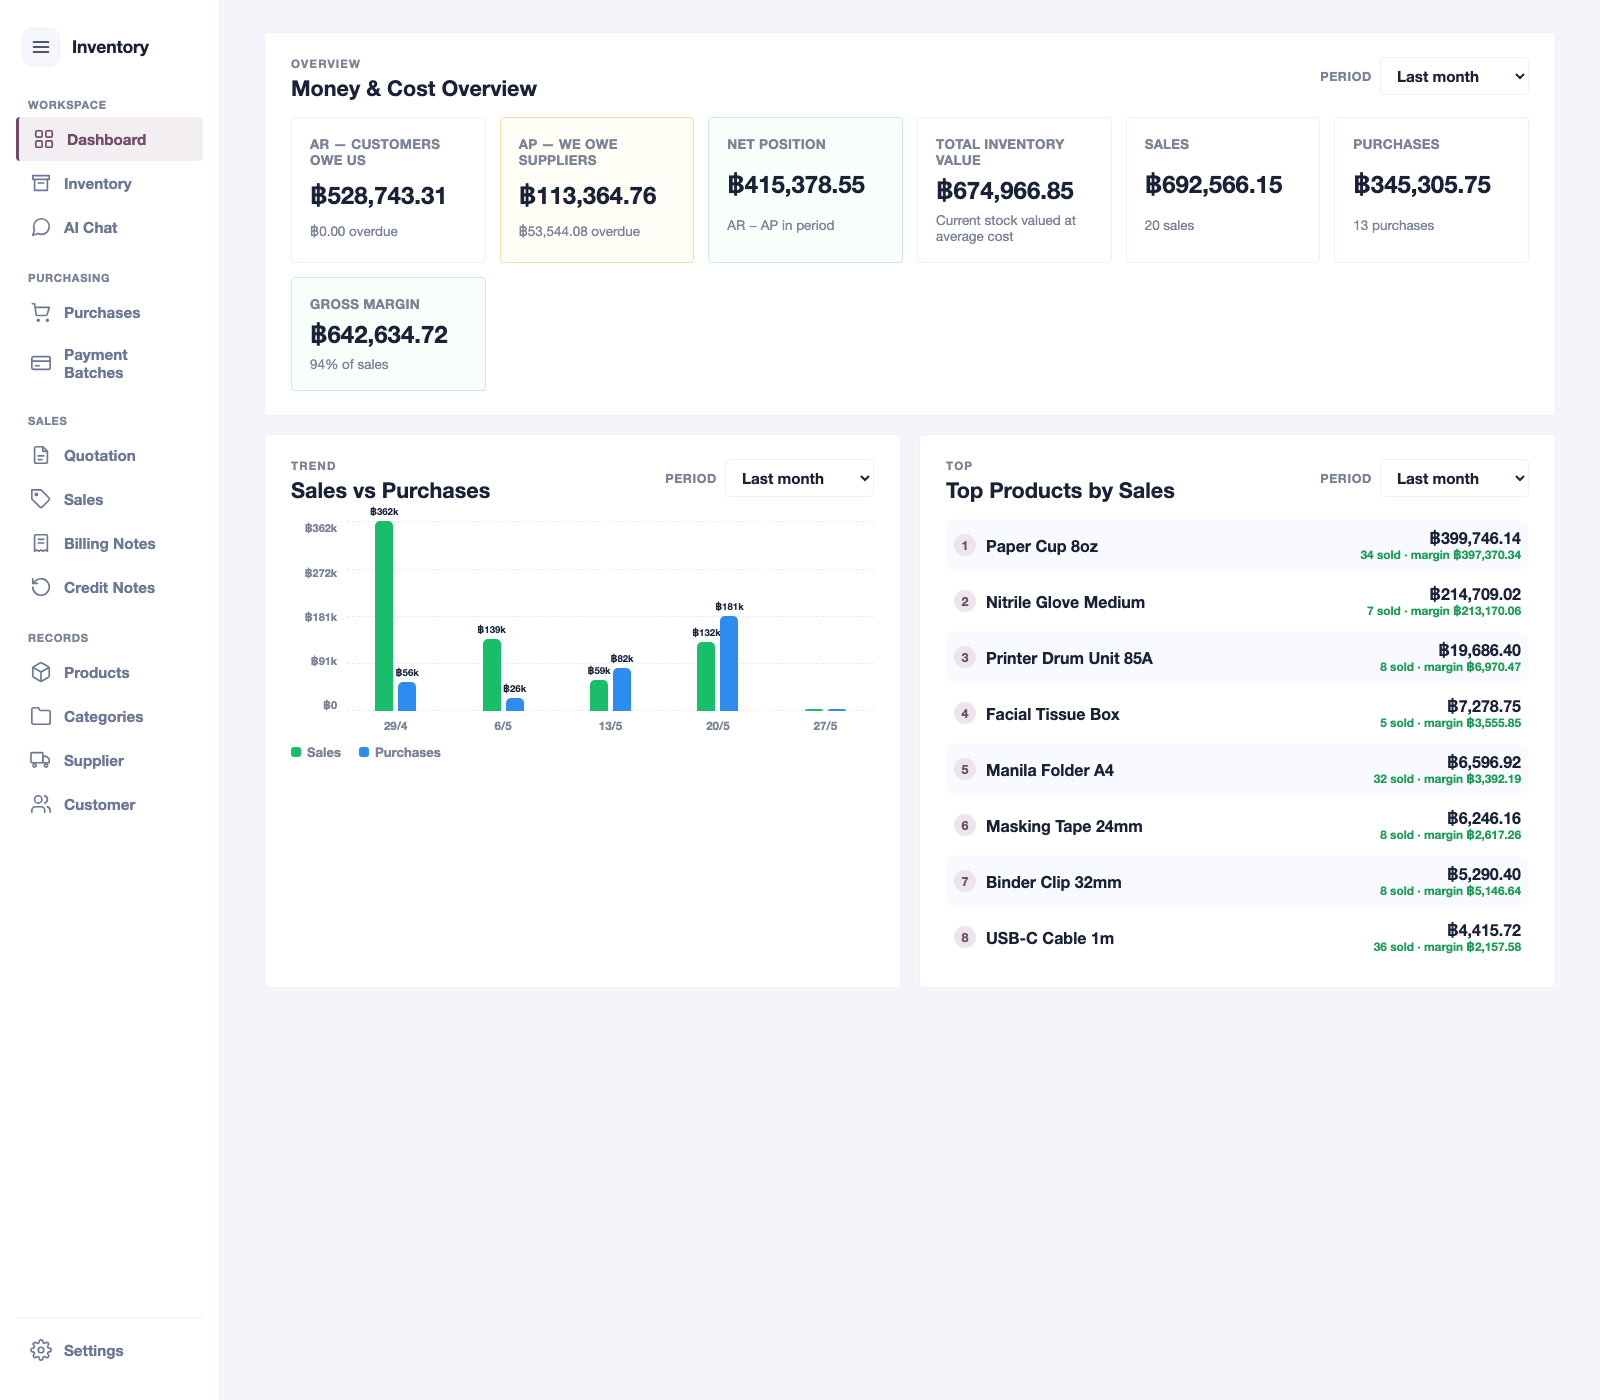
\includegraphics[width=\textwidth,height=0.55\textheight,keepaspectratio]{../docs/screenshots/sidebar-navigation.png}
	\caption{Main Sidebar Navigation}
	\label{fig:appendix-sidebar-navigation}
\end{figure}

After signing in, the sidebar is used to move between the main modules. The workspace group contains Dashboard, Inventory, AI Chat, and AI Report. The purchasing group contains Purchases and Payment Batches. The sales group contains Quotation, Sales, Billing Notes, and Credit Notes. The records group contains Products, Categories, Supplier, and Customer. Administration pages such as User Access and Activity Log are shown only to users with suitable permissions, while Settings provides the English/Thai language choice.

\section{Basic Operating Rules}

Before using the system, users should understand the following rules because they affect stock, cost, and financial records.

\begin{enumerate}
	\item Product stock is calculated from transactions. Users do not type a free stock number into the product record.
	\item Purchase items increase available stock only after the item status is changed to received.
	\item Sales items reserve or consume stock when they move into stock-affecting statuses such as packed, shipped, or delivered.
	\item The system uses first-in, first-out allocation by default, but users may choose manual stock layers when a specific received batch is physically used.
	\item Historical transactions keep snapshot information such as product names, partner names, prices, tax values, and totals. Later edits to master data should not rewrite old business documents.
	\item Billing notes, payment batches, and credit notes should be created from eligible records shown by the system instead of manually choosing unrelated transactions.
\end{enumerate}

\section{First-Time Master Data Setup}

The first step is to prepare the records that transactions depend on. Categories should be created as a clear hierarchy. Products should then be linked to the correct category and configured with SKU, base unit, purchase unit, sales unit, unit conversions, and reorder information. Suppliers and customers should also be created before purchase and sales transactions are entered.

\begin{table}[H]
	\centering
	\BlackbookTableSetup
	\caption{Master Data Setup Checklist}
	\label{tab:appendix-master-data-checklist}
	\begin{tabularx}{\textwidth}{|B{3.2cm}|Z|}
		\hline
		\textbf{Module} & \textbf{Required Setup} \\ \hline
		Categories & Create the parent and child category tree used to organize products. \\ \hline
		Products & Enter SKU, product name, category, base unit, purchase and sales units, unit conversions, reorder point, active status, and any image or PDF attachment. \\ \hline
		Suppliers & Enter supplier name, tax ID, contacts, address, payment terms, and bank or procurement details. \\ \hline
		Customers & Enter customer name, tax ID, billing address, shipping address, contacts, and payment terms. \\ \hline
	\end{tabularx}
\end{table}

\begin{figure}[!htbp]
	\centering
	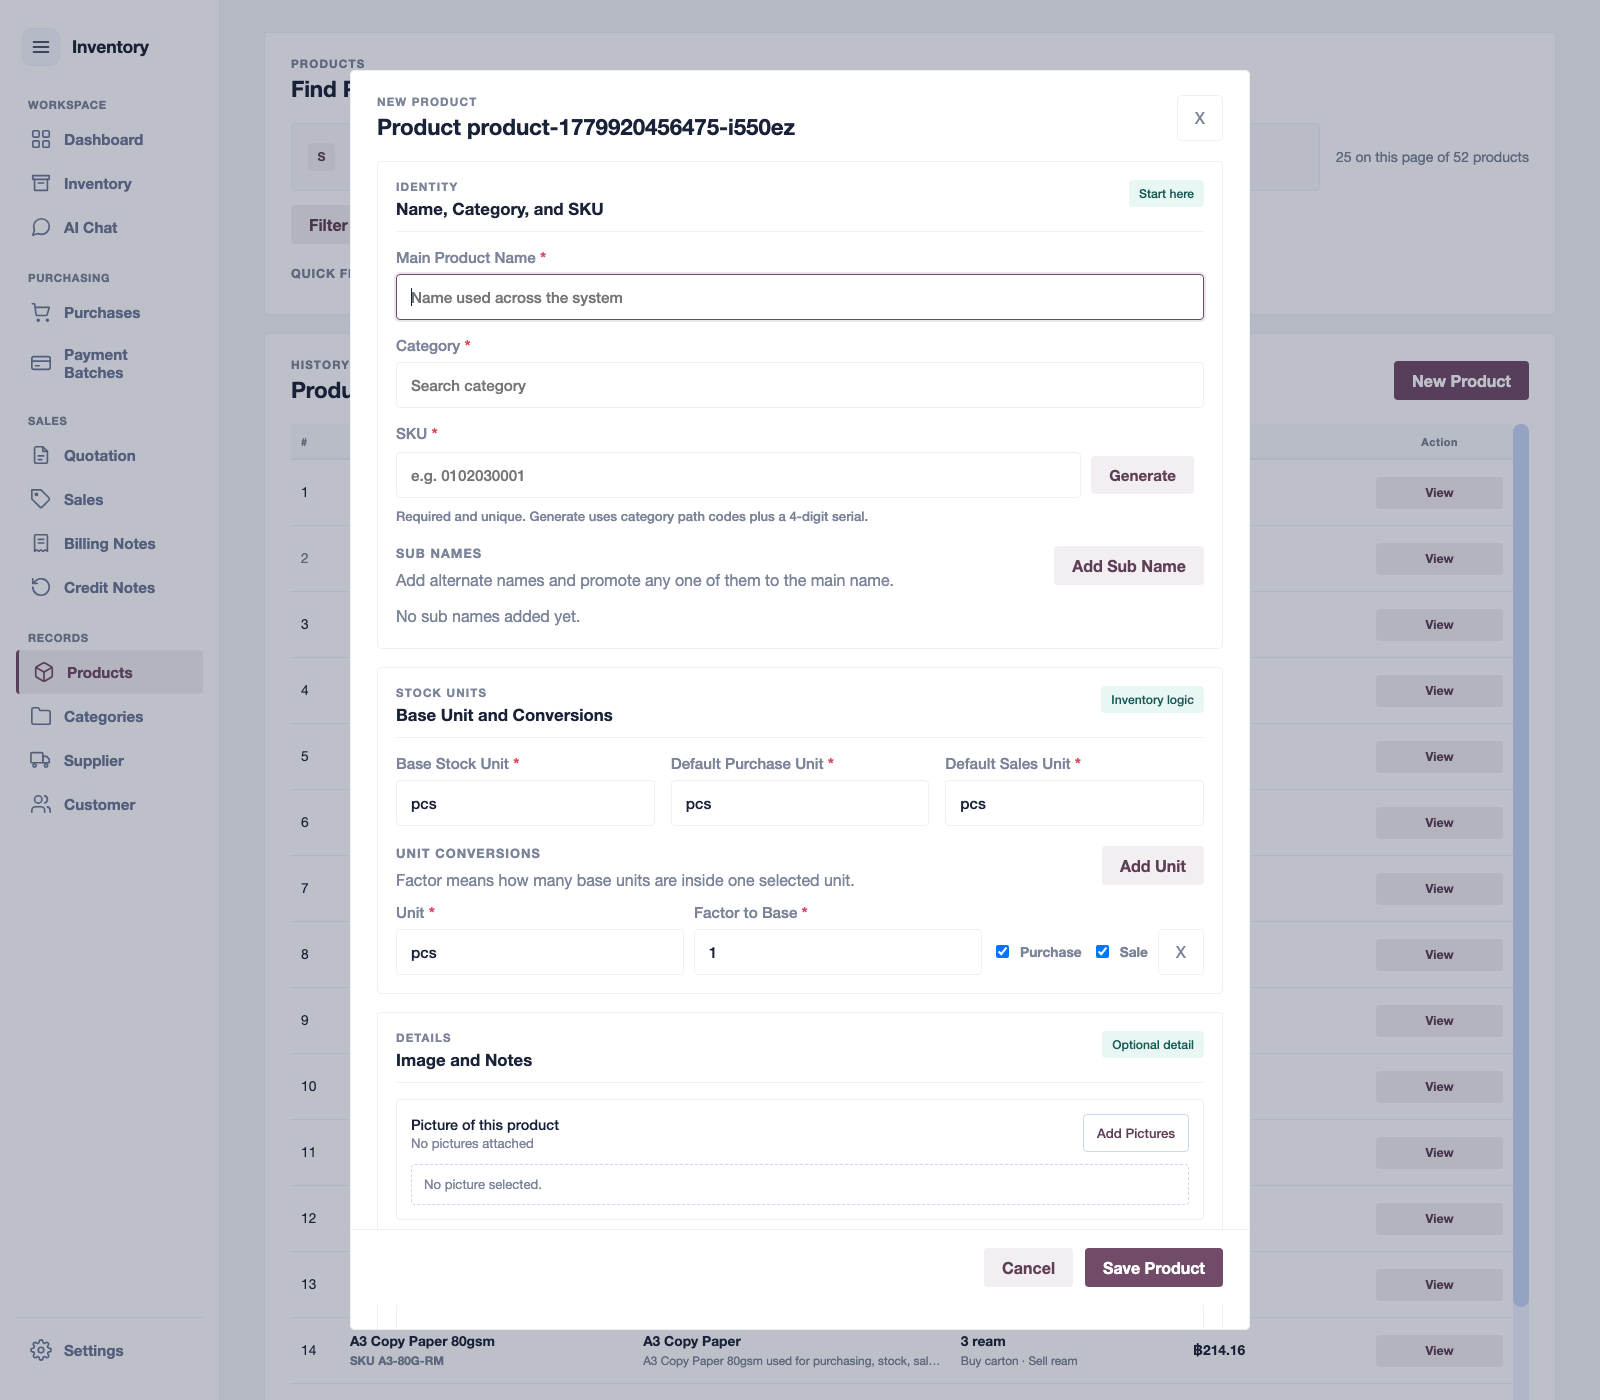
\includegraphics[width=\textwidth,height=0.55\textheight,keepaspectratio]{../docs/screenshots/product-form-unit-conversions.png}
	\caption{Product Form With Unit Conversion Setup}
	\label{fig:appendix-product-form}
\end{figure}

The base unit is especially important. It should represent the smallest unit used for stock calculation. For example, if a product is bought by box but sold by piece, the base unit may be piece and the purchase unit may be box. A conversion such as one box equals ten pieces allows the system to convert purchase quantities into stock quantities correctly.

\section{Daily Transaction Workflow}

The normal daily workflow begins with a quotation or a direct purchase or sale. A quotation records customer demand and checks whether the requested items have enough available stock. If the quotation shows that stock is short, the user can prepare a purchase from the short-stock lines. If stock is available, the user can convert the quotation into a sale.

\begin{figure}[!htbp]
	\centering
	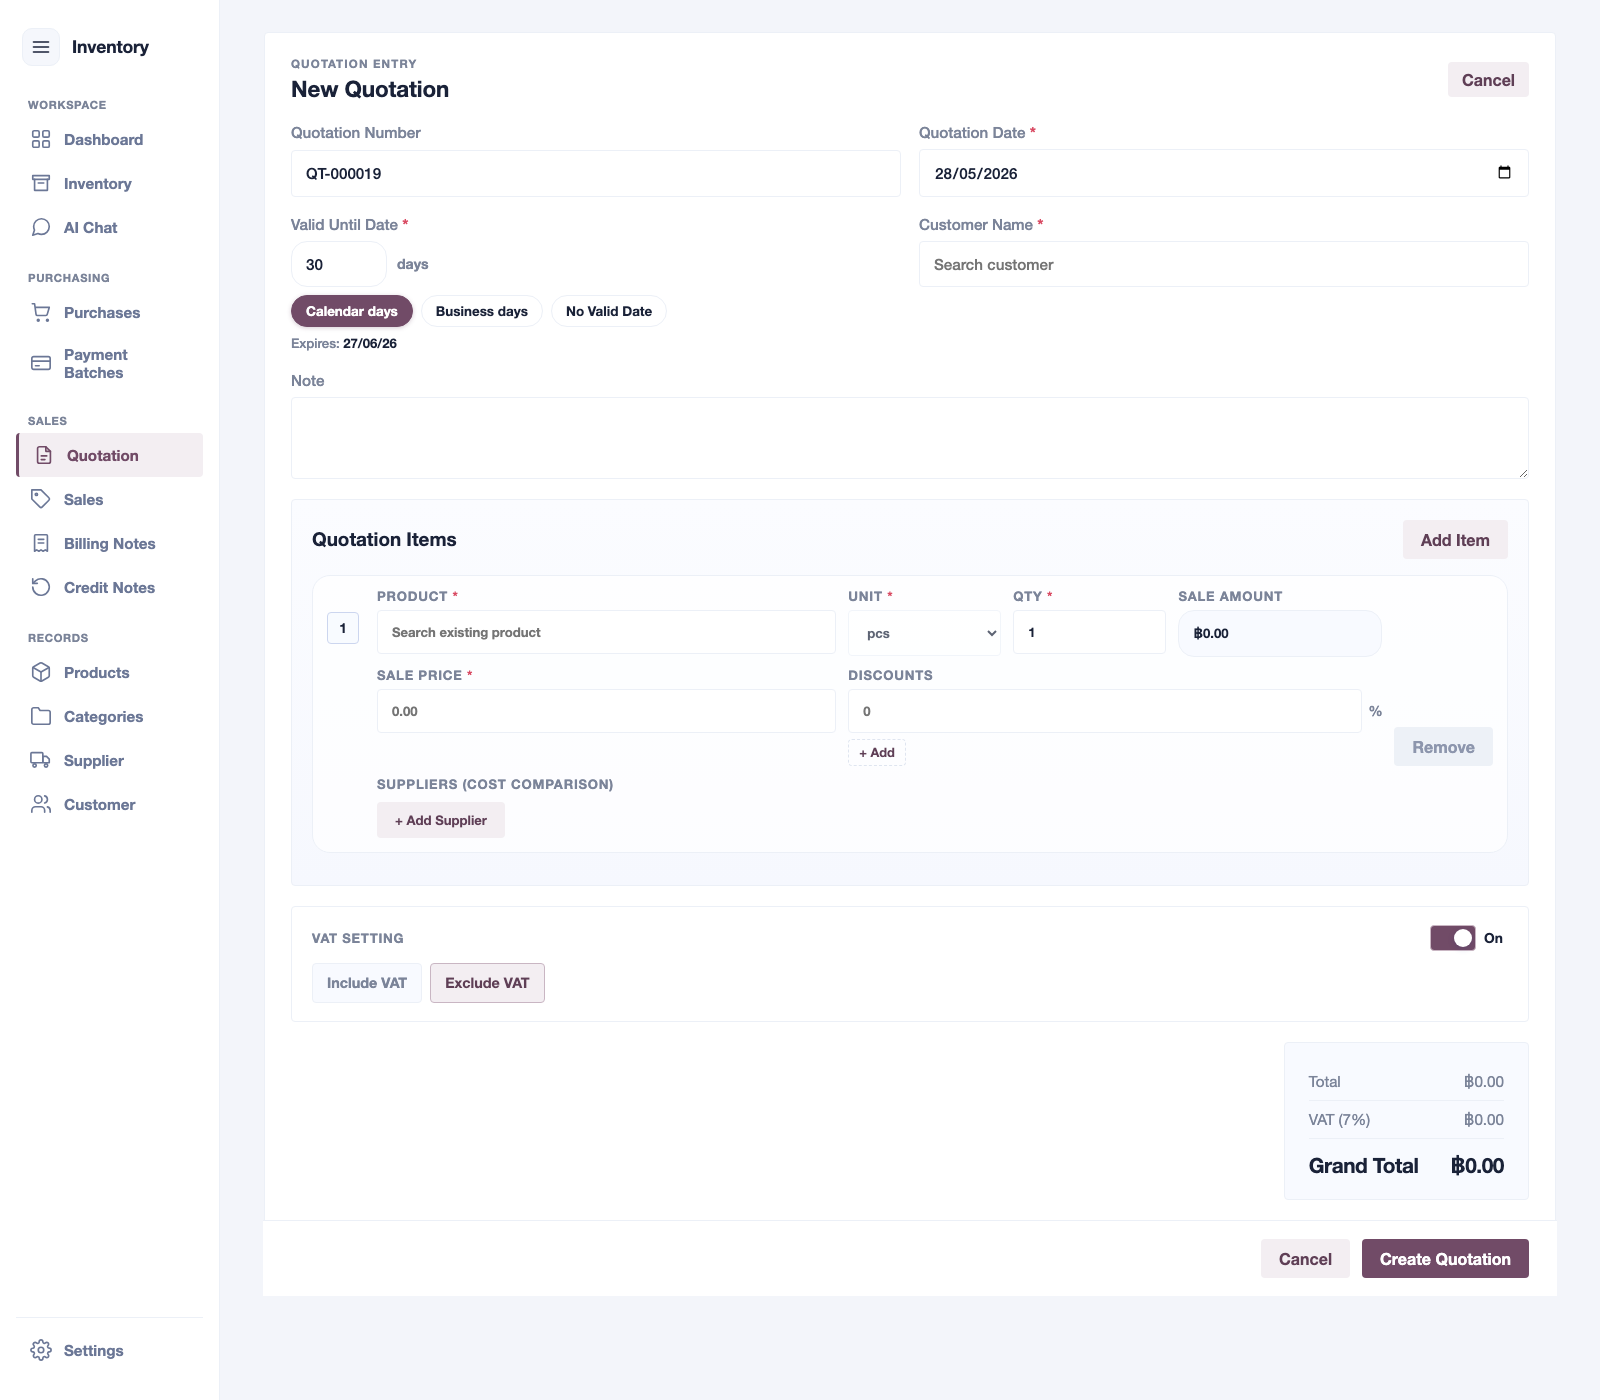
\includegraphics[width=\textwidth,height=0.55\textheight,keepaspectratio]{../docs/screenshots/quotation-entry.png}
	\caption{Quotation Entry With Stock Sufficiency Information}
	\label{fig:appendix-quotation-entry}
\end{figure}

Purchases record supplier-side orders. Users choose the supplier, add products, quantities, units, costs, and expected delivery dates, then save the purchase. When goods arrive, each purchase item should be updated to received only after the physical stock has been checked. This receiving action is what makes stock available for future sales.

\begin{figure}[!htbp]
	\centering
	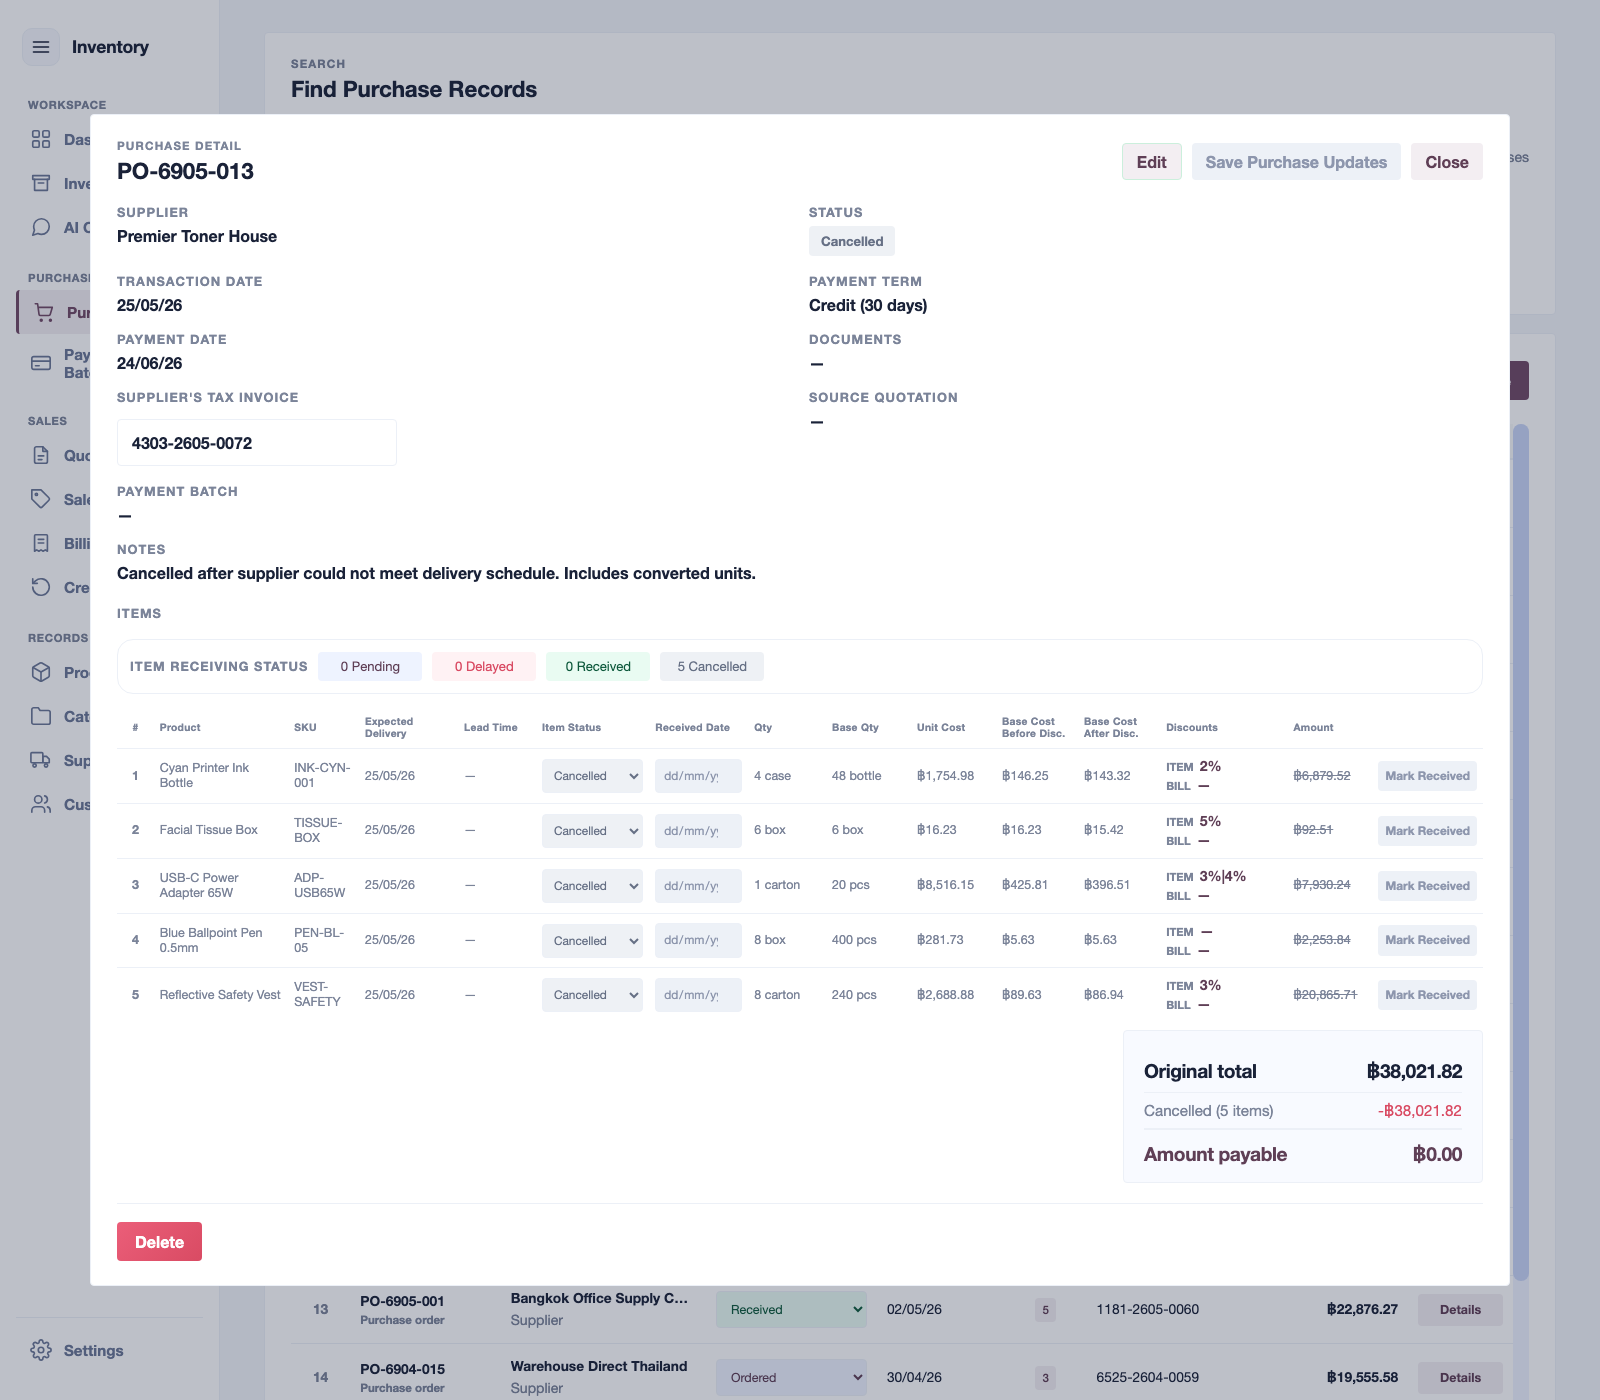
\includegraphics[width=\textwidth,height=0.55\textheight,keepaspectratio]{../docs/screenshots/purchase-form-receiving-status.png}
	\caption{Purchase Detail With Receiving Status}
	\label{fig:appendix-purchase-receiving}
\end{figure}

Sales record customer-side orders. Users choose the customer, add products, quantities, prices, and delivery-related information. The system checks stock and creates stock allocations from received purchase layers. If the user does not choose a specific layer, the system allocates stock using FIFO. Sales items should only be marked packed, shipped, delivered, cancelled, or returned when the real operational event has occurred.

\begin{figure}[!htbp]
	\centering
	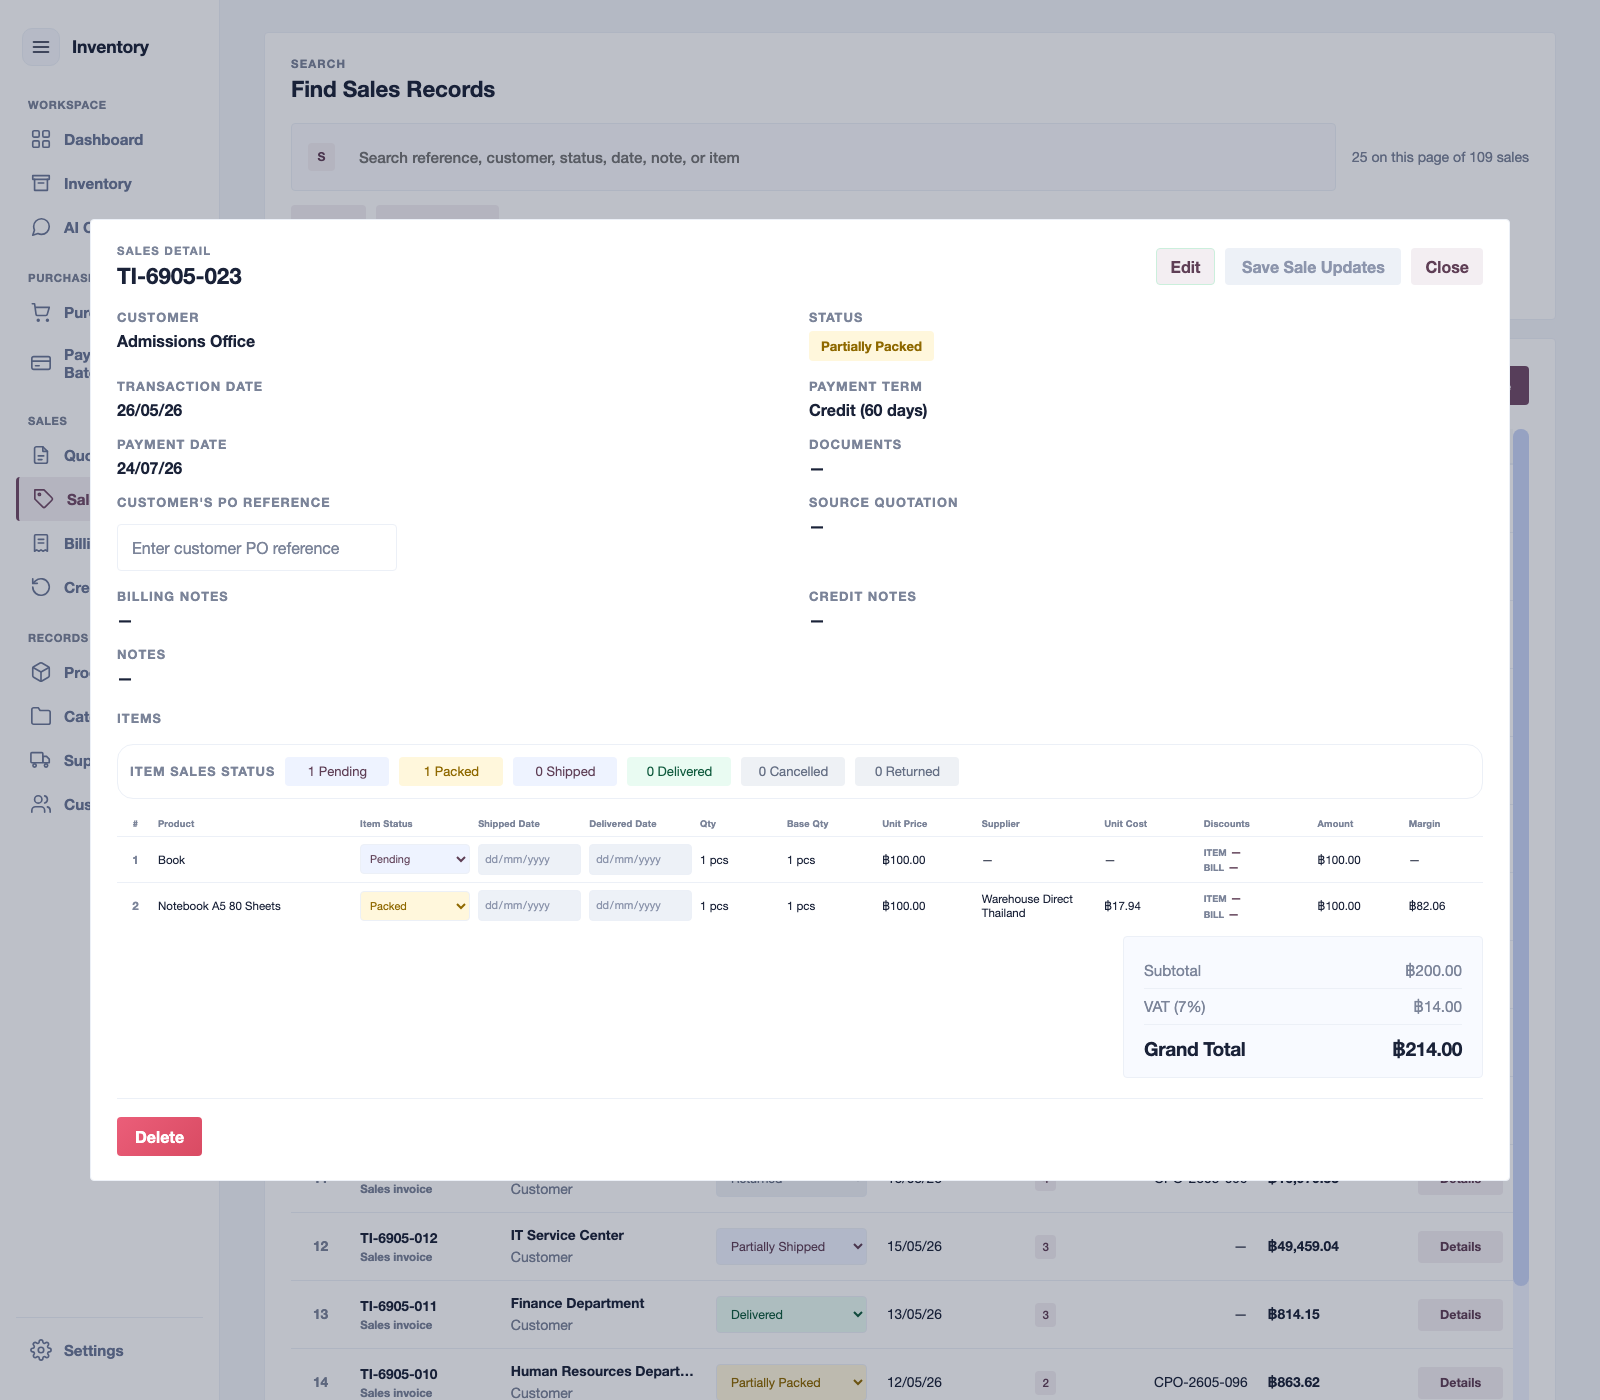
\includegraphics[width=\textwidth,height=0.55\textheight,keepaspectratio]{../docs/screenshots/sales-form-delivery-statuses.png}
	\caption{Sales Detail With Delivery Status}
	\label{fig:appendix-sales-delivery}
\end{figure}

\section{Finance Follow-Up Workflow}

Finance users use billing notes, payment batches, and credit notes to follow up completed or adjusted transactions. Billing notes group eligible customer sales for collection. Payment batches group eligible supplier purchases for payment. Credit notes record returned or cancelled sale items.

\begin{table}[H]
	\centering
	\BlackbookTableSetup
	\caption{Finance Follow-Up Modules}
	\label{tab:appendix-finance-follow-up}
	\begin{tabularx}{\textwidth}{|B{3.2cm}|B{3cm}|Z|}
		\hline
		\textbf{Module} & \textbf{Business Side} & \textbf{Main User Action} \\ \hline
		Billing Notes & Customer receivable & Select eligible shipped or delivered sales, issue the billing note, and record payment received. \\ \hline
		Payment Batches & Supplier payable & Select eligible received purchases, schedule payment, and record the paid status and bank reference. \\ \hline
		Credit Notes & Customer adjustment & Create credit notes from cancelled or returned sale items and review the tax and value adjustment. \\ \hline
	\end{tabularx}
\end{table}

These modules rely on backend eligibility checks. If a sale or purchase does not appear in the eligible list, the user should check its status, partner, and whether it has already been attached to another active document.

\section{Inventory and Business Review}

The dashboard and inventory pages are used for daily review. The dashboard summarizes urgent reorder items, stock movement, delivery planning, cash-flow pressure, popular products, and order coverage. The inventory page gives a more detailed stock-control view with product stock, pending purchases, demand, reorder values, supplier options, and product history.

\begin{figure}[!htbp]
	\centering
	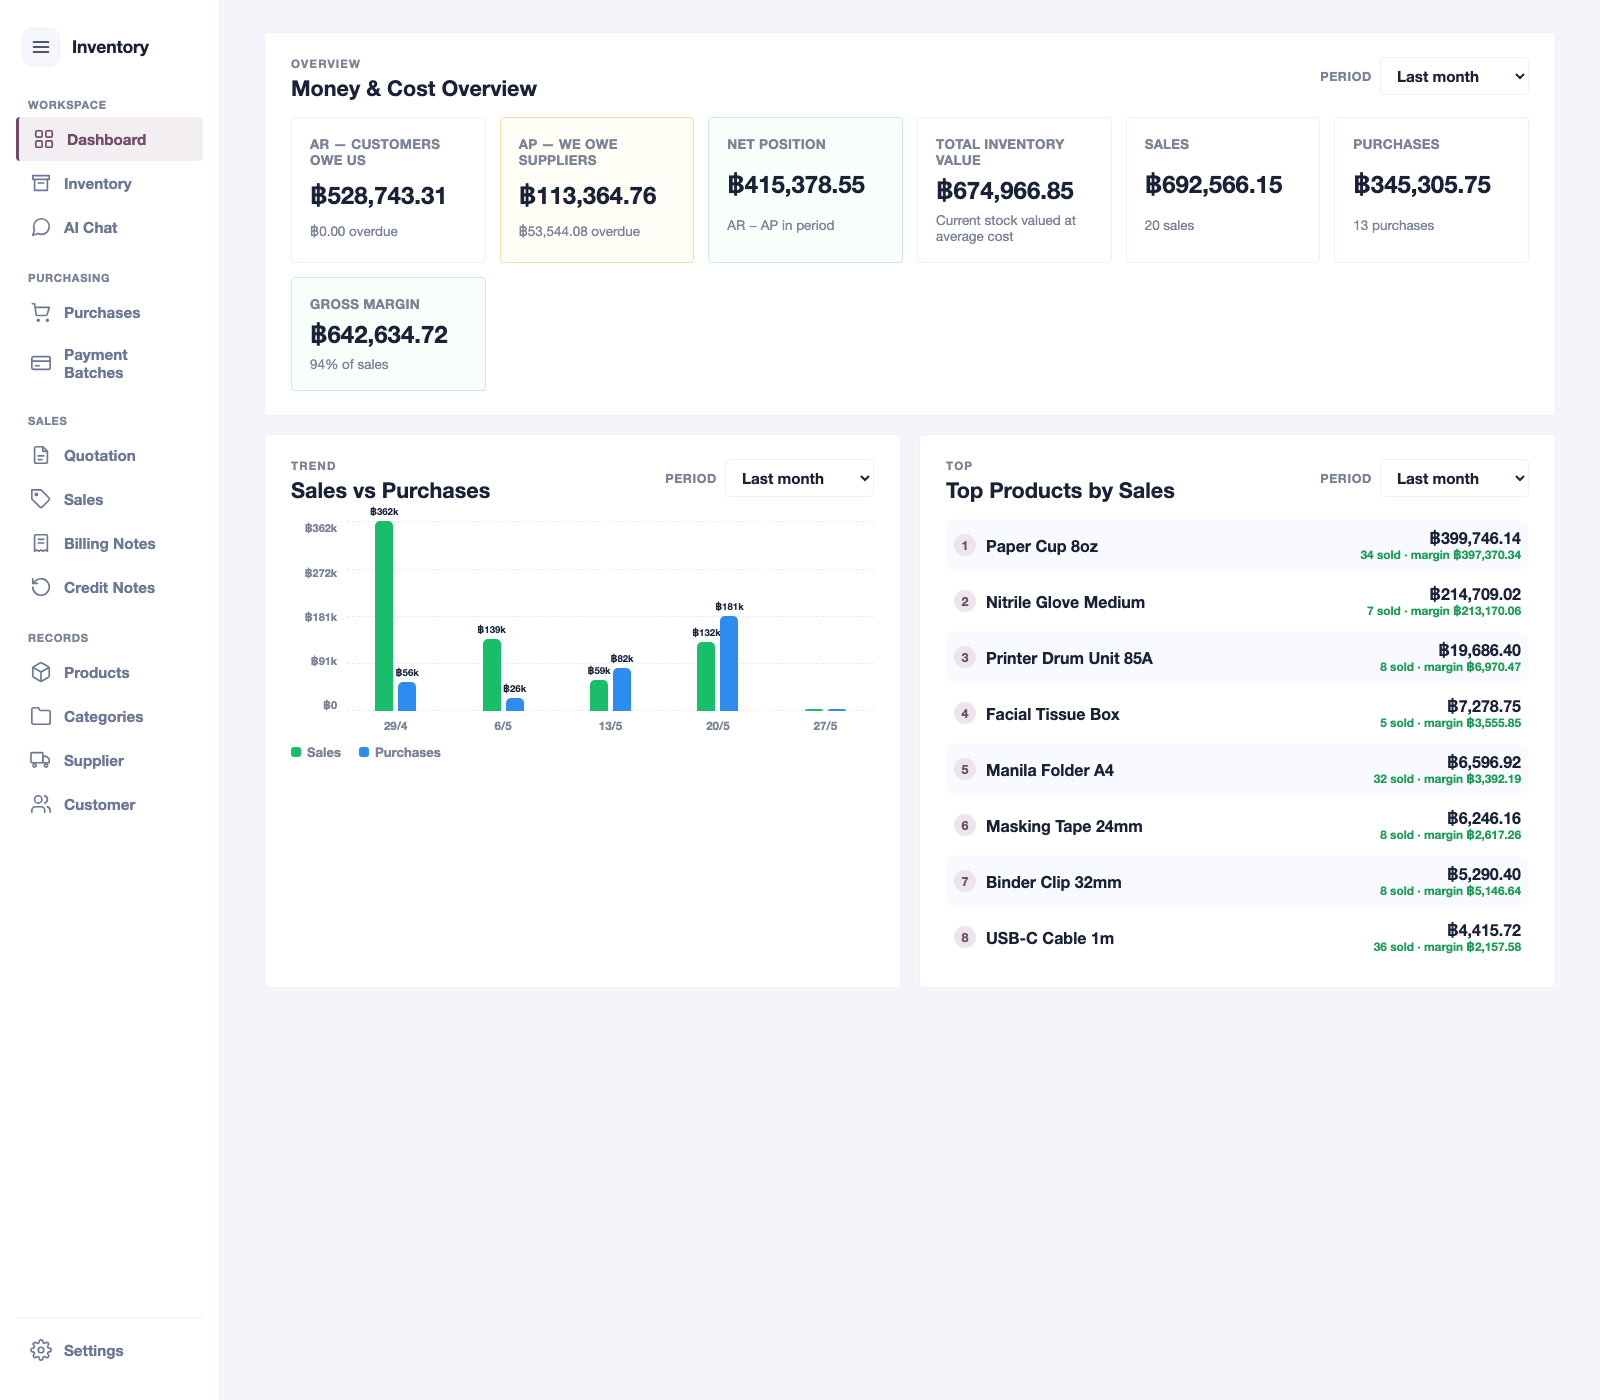
\includegraphics[width=\textwidth,height=0.55\textheight,keepaspectratio]{../docs/screenshots/dashboard-overview.png}
	\caption{Dashboard Overview for Business Review}
	\label{fig:appendix-dashboard-review}
\end{figure}

Users should review low-stock products before promising new delivery dates. They should also check delayed inbound purchases because a late supplier delivery can affect customer sales. Product history can be opened when a user needs to audit the purchase and sales records behind a stock value.

\section{AI Chat and AI Report}

AI Chat is a read-only helper for asking supported operational questions. Suitable questions include low-stock checks, supplier or customer summaries, overdue receivables, overdue payables, order coverage, and document reference lookups. With an OpenAI API key configured, the answer includes AI-written wording, a conclusion, and question-specific highlights based on the verified backend presentation. Without a key or after an API failure, the page displays the deterministic local summary. In both modes, backend data and transaction records remain the source of truth.

AI Report creates printable reports for a selected supplier, customer, or product. The user selects the report scope, selects the record, chooses a reporting period if needed, and generates the report. The generated report includes backend-prepared metrics, related records, chart data, and a written analysis. The report can be printed or saved as a PDF from the browser.

\section{Administration}

Administrators use the User Access page to create staff accounts, assign roles, activate or deactivate users, and review role permissions. The Activity Log page is used to review important system activity such as login, creation, update, and deletion events. Staff should be assigned only the access required for their responsibility.

\section{Quick Reference}

\begin{table}[H]
	\centering
	\BlackbookTableSetup
	\renewcommand{\arraystretch}{1.45}
	\caption{Quick Reference for Common User Goals}
	\label{tab:appendix-quick-reference}
	\begin{tabularx}{\textwidth}{|B{3.5cm}|B{3cm}|Z|}
		\hline
		\textbf{Goal} & \textbf{Page} & \textbf{Main Action} \\ \hline
		Check business overview & Dashboard & Review stock, delivery, receivable, payable, and coverage summaries. \\ \hline
		Check stock and reorder needs & Inventory & Filter stock rows, inspect reorder signals, and open product history. \\ \hline
		Create product records & Products & Set SKU, category, base unit, unit conversions, suppliers, and reorder information. \\ \hline
		Prepare a customer offer & Quotation & Add requested items, review stock sufficiency, and convert to purchase or sale when appropriate. \\ \hline
		Buy from supplier & Purchases & Create purchase orders and mark items received only after goods arrive. \\ \hline
		Fulfill customer order & Sales & Create sales, review FIFO allocation, and update delivery statuses. \\ \hline
		Collect customer payment & Billing Notes & Group eligible sales and record received payment. \\ \hline
		Pay supplier & Payment Batches & Group eligible purchases and record paid status. \\ \hline
		Record returns or cancellations & Credit Notes & Issue credit notes from returned or cancelled sale items. \\ \hline
		Ask operational questions & AI Chat & Ask supported read-only questions about stock, partners, AP, AR, and documents. \\ \hline
		Generate printable analysis & AI Report & Select supplier, customer, or product and generate a printable report. \\ \hline
		Manage staff access & User Access & Create users, assign roles, and review permissions. \\ \hline
		Change interface language & Settings & Switch the user interface between English and Thai. \\ \hline
	\end{tabularx}
\end{table}
